\documentclass[12pt,a4paper]{article}
\usepackage[bahasai]{babel}
\usepackage[utf8]{inputenc}
\usepackage[T1]{fontenc}
\usepackage{amsmath}
\usepackage{amssymb}
\usepackage{graphicx}
\usepackage[left=2.00cm, right=2.00cm, top=2.00cm, bottom=2.00cm]{geometry}
\title{Tugas 10 - Deret Fourier\\
	\large Mata Kuliah Sinyal dan Sistem B}


\begin{document}
	\maketitle
	\textbf{Jawab soal-soal berikut dengan baik dan benar.}
	\begin{enumerate}
		\item Berdasarkan Gambar \ref{fig:img01}, tentukan koefisien Fouriernya.
		\begin{figure}[h]
			\centering
			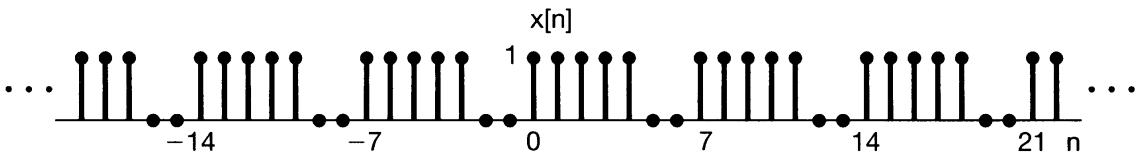
\includegraphics[width=\linewidth]{img/img01}
			\caption[shot]{Sequence $ x[n] $}
			\label{fig:img01}
		\end{figure}
		\item Berdasarkan Gambar \ref{fig:img02}, tentukan koefisien Fouriernya.
		\begin{figure}[h]
			\centering
			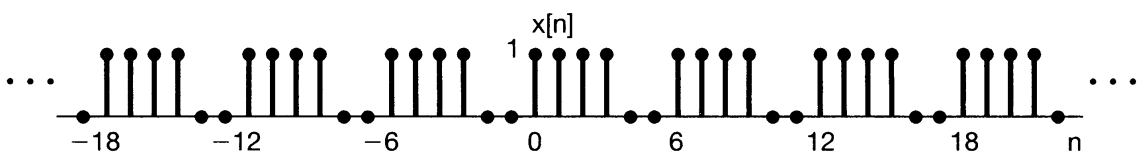
\includegraphics[width=\linewidth]{img/img02}
			\caption[shot]{Sequence $ x[n] $}
			\label{fig:img02}
		\end{figure}
		\item Berdasarkan Gambar \ref{fig:img03}, tentukan koefisien Fouriernya.
		\begin{figure}[h]
			\centering
			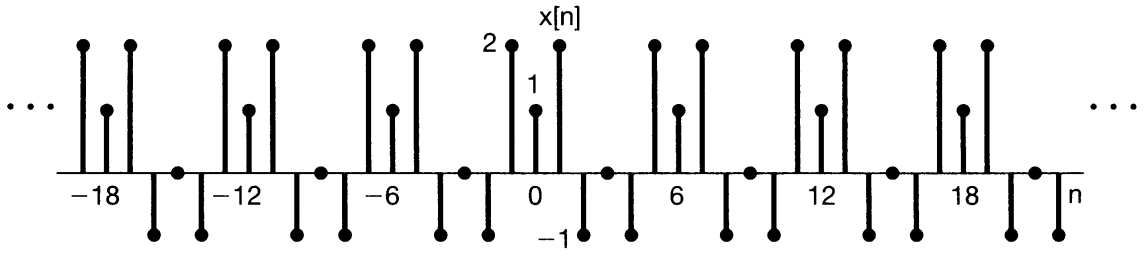
\includegraphics[width=\linewidth]{img/img03}
			\caption[shot]{Sequence $ x[n] $}
			\label{fig:img03}
		\end{figure}
		\item Tentukan representasi deret Fourier diskrit dari sequence
		\begin{equation*}
			x[n] = \cos( \pi4 n)
		\end{equation*}
		
	\end{enumerate}

	\textbf{Catatan:} Jawaban tugas dikumpulan dalam format PDF maksimal sehari sebelum perkuliahan dimulai.
\end{document}